
\documentclass[preprint,12pt]{elsarticle}

\usepackage[spanish]{babel}
\usepackage{amssymb}
\usepackage{graphicx}
\usepackage{lineno}
\usepackage[utf8]{inputenc}
\usepackage{url}
\usepackage{natbib}

\begin{document}
	
	\begin{frontmatter}

		\title{\huge  Comparativa de Cuadro de Mando Integral (BSC) y Modelo de Negocio Canvas (BMC) }
		\author{Robles Flores, Anthony Richard	                (2016056192)}
		\author{Estrella Palacios, Katherine Lizbeth			(2015050948)}
		\author{Sosa Bedoya, Sharon Fiorela				(2016054460)}
		\author{Torres Beltran , Johanna Andrea			(2020067849)}
		\address{Tacna, Perú}
		


%%INICIO abstract
\begin{abstract}

\end{abstract}
%%FIN abstract


\end{frontmatter}

%%INICIO Resumen
\section{Resumen}

%%FIN Resumen


%%INICIO Introducción
\section{Introducción}


%%FIN Introducción


%%INICIO Marco Teórico
\section{Marco Teórico}

%%----------------------------------------------------------------------------------------------------------------------------------------------------------
	\subsection{\textbf{Cuadro de Mando Integral (BSC)}}
	
xxxxxxxxxxxxxxxxxxxxxxxxxxxxxxxxxxxxxxxxxxxxxxxxxxxxxxxxxxxxxxxxxxxxxxxxxxxxxxxxxxxxxxxxxxx\cite{referenciarobles1}

\subsubsection{\textbf{Subtitulo 1}}

	\begin{itemize}
	\item a
	\item b
	\item c
	\end{itemize}



\subsubsection{\textbf{Propuesta de Valor al Cliente}}

%%https://www.grandespymes.com.ar/2011/06/13/balanced-scorecard-cuadro-de-mando-integral/

Dado que el BSC ha de ser sencillo y fácilmente entendible, es clave seleccionar aquellos objetivos estratégicos de primer nivel que son prioritarios. Para ello, resulta de gran utilidad definir la propuesta de valor al cliente, es decir, lo que diferencia a nuestra organización ante los clientes. Diferentes gurús de la estrategia han distinguido formas de competir. Kaplan y Norton las resumen, siguiendo la clasificación de Trecy y Weserman, en:

	\begin{itemize}
	\item Liderazgo de productos: se centra en la excelencia de sus productos y servicios, que ofrecen la máxima calidad y funcionalidad.
	\item Relación con el cliente: se centra en la capacidad para generar vínculos con los clientes, para conocerlos y proporcionarles productos y servicios adecuados a sus necesidades.
	\item Excelencia operativa: se centra en proporcionar productos y servicios a un precio competitivo para la calidad y funcionalidad que ofrecen.
	\end{itemize}

Las organizaciones intentan ser excelentes en una de esas estrategias, manteniendo unos estándares mínimos en las otras dos. Es lógico que las perspectivas del cliente y, por ende, las  de procesos y aprendizaje y crecimiento, se centren en objetivos relacionados con la estrategia para los que no se ha conseguido el mínimo requerido.

\subsubsection{\textbf{Indicadores y sus Metas}}

Los indicadores (también llamados medidas) son el medio que tenemos para visualizar si estamos cumpliendo o no los objetivos estratégicos.

Un objetivo estratégico, como por ejemplo el desarrollo de capacidades comerciales de nuestro personal clave, puede medirse a través de indicadores.
\\

Se pueden establecer dos tipos de indicadores:

	\begin{itemize}
	\item Indicadores de resultado: miden la consecuencia del objetivo estratégico. También se les llama indicadores de efecto.
	\item Indicadores de causa: miden el resultado de las acciones que permiten su consecución. También se llaman indicadores inductores.
	\end{itemize}

Las organizaciones intentan ser excelentes en una de esas estrategias, manteniendo unos estándares mínimos en las otras dos. Es lógico que las perspectivas del cliente y, por ende, las  de procesos y aprendizaje y crecimiento, se centren en objetivos relacionados con la estrategia para los que no se ha conseguido el mínimo requerido.

\subsubsection{\textbf{Iniciativas Estratégicas}}

Las iniciativas estratégicas son las acciones en las que la organización se va a centrar para la consecución de los objetivos estratégicos. En nuestras empresas hacemos cosas, pero ¿están realmente enfocadas hacia el cumplimiento de la estrategia? En muchas organizaciones encontramos un exceso de iniciativas y proyectos con falta de recursos y tiempo para llevarlos a cabo.
\\

Es importante priorizar las iniciativas en función de los objetivos estratégicos. Si analizamos el impacto de las iniciativas en marcha en cada uno de los objetivos estratégicos, podemos visualizar, iniciativas que aportan poco valor al cumplimiento de estos objetivos y objetivos estratégicos sin soporte a las iniciativas

\subsubsection{\textbf{Responsables y Recursos}}

Cada objetivo, indicador e iniciativa debe tener un responsable. Una persona a cargo que controla su cumplimiento.
\\
Otro aspecto clave para una implantación con éxito del BSC es asignar los recursos necesarios para el buen desarrollo de las iniciativas estratégicas. Es el primer paso para el cumplimiento de la estrategia. Por ello es necesario establecer los equipos a cargo de cada iniciativa, así como el papel que diferentes personas van a jugar en ellos. Y también dotar a las iniciativas de los recursos necesarios para su cumplimiento. Se recomienda que el presupuesto contenga una partida de recursos asignados a las iniciativas estratégicas. Estos recursos deben estar diferenciados del presupuesto operativo, del presupuesto de inversión y de otros presupuestos que utilizan las empresas, asi podemos evitar que otras actividades engullan esos recursos que debieran dedicarse al cumplimiento de las iniciativas críticas definidas en el BSC.

\subsubsection{\textbf{Características del Cuadro de Mando Integral}}

El desarrollo de un sistema integral de gerencia requiere un sistema balanceado de indicadores. El sistema reconoce la causa y efecto entre acciones y resultados. Reconoce que para deleitar a un inversionista, la empresa tiene que ser rentable. Reconoce que para hacer feliz al cliente necesita reducir o eliminar costos y mejorar la calidad del producto o servicio. Para mantener la ventaja competitiva a largo plazo, es necesario aprender y aprender y a innovar. El Balanced Scorecard tiene las siguientes características:


	\begin{itemize}
	\item Articula los factores que impulsan la estrategia de la organización.
	\item Le pone brazos y manos a la visión/misión.

	\item Permite, de forma concreta, entender la razón de ser de la organización y sus metas
	\item Define en concreto las metas críticas para alcanzar el éxito.

	\item Permite su difusión a lo largo y ancho de la organización.
	\item Define el desarrollo de indicadores de desempeño para cada meta.

	\item Asegura que todos entienden los indicadores de las áreas y de la empresa en general.
	\item Comunica cómo estos están interrelacionados.

	\item Conecta cada medida a un sistema de retroalimentación formal.
	\item Integra la comunicación con la regularidad.

	\item Integra la comunicación con la regularidad.
	\end{itemize}

%%----------------------------------------------------------------------------------------------------------------------------------------------------------

	\subsection{\textbf{Modelo de Negocio Canvas (BMC) }}
	
xxxxxxxxxxxxxxxxxxxxxxxxxxxxxxxxxxxxxxxxxxxxxxxxxxxxxxxxxxxxxxxxxxxxxxxxxxxxxxxxxxxxxxxxxxxxxxxxxxxxxxxxxxxx

	\subsubsection{\textbf{Subtitulo 1}}
	\begin{itemize}
	\item{\textbf{1. Punto1: }}XXXXXXXXXXXXX
	\item {\textbf{2. Punto2: }}XXXXXXXXXXXX
	\item {\textbf{3. Punto3: }}XXXXXXXXXXXX
	\end{itemize}

	\subsubsection{\textbf{Subtitulo 2}}

	\begin{itemize}
	\item a
	\item b
	\item c
	\end{itemize}

	\subsubsection{\textbf{Subtitulo 3}}

	\begin{figure}[htb]
		\begin{center}
			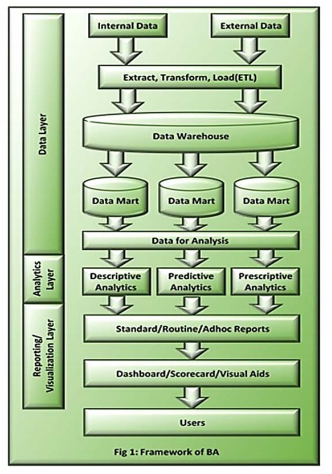
\includegraphics[height=9cm]{./IMAGENES/BAFramework} 
			\caption{Framework de BA}
		\end{center}
	\end{figure}


%%FIN Marco Teórico
%%----------------------------------------------------------------------------------------------------------------------------------------------------------


%COMPRACION

\section{Comparación entre Cuadro de Mando Integral (BSC) y Modelo de Negocio Canvas (BMC)}
A continuación se muestra la comparación entre Cuadro de Mando Integral (BSC) y Modelo de Negocio Canvas (BMC)
	
	\begin{itemize}

	\item{\textbf{1.}} XXXXXXXXXXXXXXXXXXXX
	\item{\textbf{2.}} XXXXXXXXXXXXXXXXXXXX
	\item{\textbf{3.}} XXXXXXXXXXXXXXXXXXXX
	\item{\textbf{4.}} XXXXXXXXXXXXXXXXXXXX
	\item{\textbf{5.}} XXXXXXXXXXXXXXXXXXXX
	\item{\textbf{6.}} XXXXXXXXXXXXXXXXXXXX
	\item{\textbf{7.}} XXXXXXXXXXXXXXXXXXXX
	\end{itemize}

%%----------------------------------------------------------------------------------------------------------------------------------------------------------

%CONCLUSIONES
\section{Conclusiones}

%%****
	\begin{itemize}
		\item XXXXXXXXXXXXXXXXXXXX
		\item XXXXXXXXXXXXXXXXXXXX
		\item XXXXXXXXXXXXXXXXXXXX
	\end{itemize}

%%----------------------------------------------------------------------------------------------------------------------------------------------------------

%RECOMENDACIONES
\section{Recomendaciones}	

	\begin{itemize}
		\item XXXXXXXXXXXXXXXXXXXX
		\item XXXXXXXXXXXXXXXXXXXX
		\item XXXXXXXXXXXXXXXXXXXX
	\end{itemize}


%%----------------------------------------------------------------------------------------------------------------------------------------------------------

	
	\newpage
	\bibliographystyle{apalike}
	\bibliography{BIBLIOGRAFIA}	



\end{document}

